\documentclass[12pt,a4paper]{extarticle}
\usepackage[utf8]{inputenc}
\usepackage[T5]{fontenc}
\usepackage{geometry}
\geometry{a4paper, left=1.5cm, right=1cm, top=1.5cm, bottom=1.5cm, headheight=20pt, headsep=15pt, footskip=28pt}
\usepackage{enumitem}
\usepackage{amsmath}
\usepackage{amssymb}
\usepackage{diagbox}
\usepackage{colortbl} % Sửa lỗi \arrayrulecolor
\usepackage{array}    % Hỗ trợ định dạng cột m{2cm}
\usepackage[most]{tcolorbox}
\newcommand{\khongxacdinh}{\text{KXĐ}}
\newcommand{\blackbox}[1]{\texorpdfstring{\fcolorbox{black}{black}{\textcolor{white}{#1}}}{#1}}
\usepackage{tikz}
\definecolor{bookblue}{RGB}{58,90,172}
\definecolor{book}{RGB}{58,90,172}
\definecolor{myblue}{RGB}{200,40,40}
\newcommand{\bluecheck}{\textcolor{myblue}{\checkmark}}
\newtcolorbox{formulaBox}{colback=gray!5,colframe=bookblue,boxrule=0.8pt,arc=2mm}
\newtcolorbox{notebox}{colback=blue!3,colframe=myblue,boxrule=0.8pt,arc=2mm}
\usetikzlibrary{patterns, patterns.meta} % Thêm patterns.meta vào đây
% Gọi package nằm trong thư mục con template
\usepackage{../template/mngocbox}

\begin{document}

% Sử dụng ngoặc vuông [...] để thay đổi linh hoạt các thông số
\makeheadbox[headerright={Chương 2},chude={Bài 2},tieude={Toạ độ Vector},dinhdang={Hình học},lop={12 },gv={Nguyễn Lê Minh Ngọc}]
\vspace{2em}
\makeheading{I}{Kiến thức cần nhớ}
\section*{A. Kiến thức cần nhớ về tọa độ vectơ}
\begin{center}
    \begin{minipage}{0.48\textwidth}
        \centering
        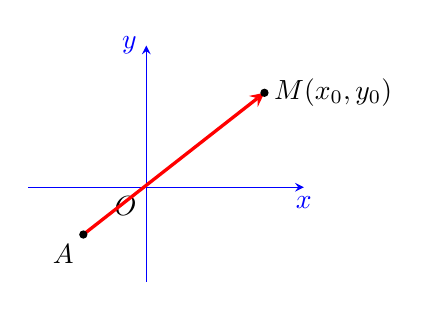
\begin{tikzpicture}[scale=1.0, >=stealth]
            % Axes
            \draw[->, blue] (-1.5, 0) -- (2.0, 0) node[below] {$x$};
            \draw[->, blue] (0, -1.2) -- (0, 1.8) node[left] {$y$};
            \node[below left] at (0,0) {$O$};
            
            % Vector AM
            \coordinate (A) at (-0.8, -0.6);
            \coordinate (M) at (1.5, 1.2);
            
            \draw[->, red, very thick] (A) -- (M);
            \fill (A) circle (1.5pt) node[below left] {$A$};
            \fill (M) circle (1.5pt) node[right] {$M(x_0, y_0)$};
        \end{tikzpicture}
    \end{minipage}
    \hfill
    \begin{minipage}{0.48\textwidth}
        \vspace{1cm}
        \textbf{Lớp 10:}
        \[
        \vec{AB} = (x_B - x_A; y_B - y_A)
        \]
    \end{minipage}
\end{center}
\vspace{1.5em}
\subsection*{1) Hệ trục tọa độ trong không gian}
\begin{center}
    \begin{minipage}{0.45\textwidth}
        \centering
        \begin{tikzpicture}[scale=1.2, >=stealth]
            % 3D Axes
            \draw[->, thick, blue] (0,0) -- (0,2.2) node[above] {$z$};
            \draw[->, thick, blue] (0,0) -- (2.2,0) node[right] {$y$};
            \draw[->, thick, blue] (0,0) -- (-1.1,-1.1) node[left] {$x$};
            \node[below left] at (0,0) {$O$};
            
            % Unit vectors
            \draw[->, red, very thick] (0,0) -- (0,0.8) node[left] {$\vec{k}$};
            \draw[->, red, very thick] (0,0) -- (0.8,0) node[above] {$\vec{j}$};
            \draw[->, red, very thick] (0,0) -- (-0.45,-0.45) node[left] {$\vec{i}$};
        \end{tikzpicture}
    \end{minipage}
    \hfill
    \begin{minipage}{0.5\textwidth}
        Hệ gồm 3 trục $Ox$, $Oy$, $Oz$ đôi một vuông góc với nhau gọi là \textbf{hệ tọa độ vuông góc $Oxyz$ trong không gian}, hay gọi tắt là \textbf{Hệ tọa độ $Oxyz$}.
        
        \vspace{0.8em}
        Không gian với hệ tọa độ $Oxyz$ gọi là: \textbf{Không gian $Oxyz$}.
    \end{minipage}
\end{center}
\vspace{1em}
\begin{itemize}[leftmargin=*, label=$\bullet$, itemsep=0.4em]
    \item Trục hoành: $Ox$
    \item Trục tung: $Oy$
    \item Trục cao: $Oz$
    \item Các mặt phẳng $(Oxy)$, $(Oyz)$, $(Ozx)$ là các \textbf{mặt phẳng tọa độ}.
\end{itemize}
\vspace{1.5em}
\subsection*{2) Tọa độ của một điểm}
\begin{center}
    \begin{minipage}{0.45\textwidth}
        \centering
        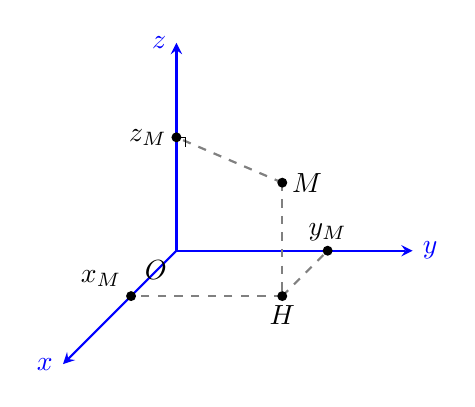
\begin{tikzpicture}[scale=1.2, >=stealth]
            % 3D Axes
            \draw[->, thick, blue] (0,0) -- (0,2.2) node[left] {$z$};
            \draw[->, thick, blue] (0,0) -- (2.5,0) node[right] {$y$};
            \draw[->, thick, blue] (0,0) -- (-1.2,-1.2) node[left] {$x$};
            \node[below left] at (0,0) {$O$};
            
            % Coordinates representation
            \coordinate (M) at (1.12, 0.72);
            \coordinate (H) at (1.12, -0.48);
            \coordinate (Mz) at (0, 1.2);
            \coordinate (Mx) at (-0.48, -0.48);
            \coordinate (My) at (1.6, 0);
            
            % Projections
            \draw[dashed, thick, gray] (M) -- (H);
            \draw[dashed, thick, gray] (M) -- (Mz);
            \draw[dashed, thick, gray] (H) -- (Mx);
            \draw[dashed, thick, gray] (H) -- (My);
            
            % Right angle indicator at Mz
            \draw (0, 1.2) -- (0.1, 1.2) -- (0.1, 1.1);
            
            % Points and Labels
            \fill (M) circle (1.5pt) node[right] {$M$};
            \fill (H) circle (1.5pt) node[below] {$H$};
            \fill (Mz) circle (1.5pt) node[left] {$z_M$};
            \fill (Mx) circle (1.5pt) node[above left] {$x_M$};
            \fill (My) circle (1.5pt) node[above] {$y_M$};
        \end{tikzpicture}
    \end{minipage}
    \hfill
    \begin{minipage}{0.5\textwidth}
        \textbf{Để tìm tọa độ điểm $M$ trong không gian:}
        \begin{enumerate}[label=\textbf{Bước \arabic*.}, leftmargin=*]
            \item Xác định hình chiếu của $M$ lên mặt phẳng $(Oxy)$, gọi là $H$.
            \item Xác định tọa độ của $H$ trên mặt phẳng $(Oxy)$:
            \[
            x_H = x_M; \quad y_H = y_M
            \]
            \item Xác định hình chiếu của $M$ lên trục $Oz$, gọi là $M_z$:
            \[
            z_M = z_{M_z}
            \]
        \end{enumerate}
    \end{minipage}
\end{center}
\vspace{1em}
\noindent Bộ số $(x_M; y_M; z_M)$ là tọa độ của điểm $M$ trong không gian $Oxyz$, ký hiệu là $M(x_M; y_M; z_M)$.
\vspace{1.5em}
\noindent $\blacktriangleright$ \textbf{Chú ý:}
\begin{itemize}[leftmargin=*, label=$\circ$]
    \item Tọa độ của điểm $M$ trong không gian $Oxyz$ là \textbf{duy nhất}.
    \item Người ta có thể xác định tọa độ điểm $M$ bằng cách xác định trực tiếp hình chiếu của $M$ lên các trục tọa độ.
\end{itemize}
\subsection*{3) Tọa độ của vectơ}

\noindent Trong không gian $Oxyz$, cho vectơ $\vec{u}$. Xét điểm $M$ thỏa mãn $\vec{OM} = \vec{u}$. Khi đó, tọa độ của điểm $M$ chính là tọa độ của vectơ $\vec{u}$.

\begin{center}
    \begin{minipage}{0.45\textwidth}
        \centering
        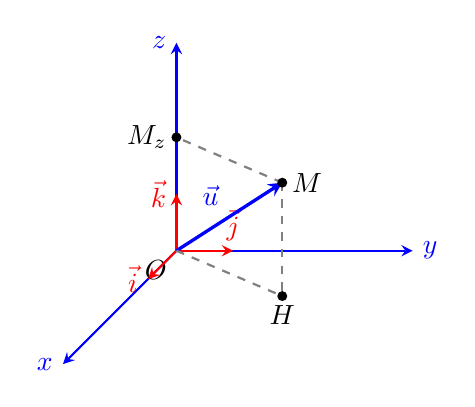
\begin{tikzpicture}[scale=1.2, >=stealth]
            % 3D Axes
            \draw[->, thick, blue] (0,0) -- (0,2.2) node[left] {$z$};
            \draw[->, thick, blue] (0,0) -- (2.5,0) node[right] {$y$};
            \draw[->, thick, blue] (0,0) -- (-1.2,-1.2) node[left] {$x$};
            \node[below left] at (0,0) {$O$};
            
            % Unit vectors
            \draw[->, red, thick] (0,0) -- (0,0.6) node[left] {$\vec{k}$};
            \draw[->, red, thick] (0,0) -- (0.6,0) node[above] {$\vec{j}$};
            \draw[->, red, thick] (0,0) -- (-0.3,-0.3) node[left] {$\vec{i}$};
            
            % Coordinates representation
            \coordinate (M) at (1.12, 0.72);
            \coordinate (H) at (1.12, -0.48);
            \coordinate (Mz) at (0, 1.2);
            
            % Vector u = OM
            \draw[->, blue, very thick] (0,0) -- (M) node[midway, above left] {$\vec{u}$};
            
            % Projections
            \draw[dashed, thick, gray] (M) -- (H);
            \draw[dashed, thick, gray] (M) -- (Mz);
            \draw[dashed, thick, gray] (0,0) -- (H);
            
            % Points and Labels
            \fill (M) circle (1.5pt) node[right] {$M$};
            \fill (H) circle (1.5pt) node[below] {$H$};
            \fill (Mz) circle (1.5pt) node[left] {$M_z$};
        \end{tikzpicture}
    \end{minipage}
    \hfill
    \begin{minipage}{0.5\textwidth}
        Nếu $M(a; b; c)$ thì $\vec{u} = (a; b; c)$.
        
        \vspace{0.8em}
        Ký hiệu: $\vec{u} = (a; b; c)$ hoặc $\vec{u}(a; b; c)$.
        
        \vspace{0.8em}
        Nếu $\vec{i}, \vec{j}, \vec{k}$ là các vectơ đơn vị trên các trục $Ox, Oy, Oz$ và $\vec{u} = (a; b; c)$ thì:
        \[
        \vec{u} = a\vec{i} + b\vec{j} + c\vec{k}
        \]
    \end{minipage}
\end{center}

\vspace{2em}

\subsection*{$\bigstar$ Hai vectơ bằng nhau}

\noindent Cho $\vec{u} = (a; b; c)$ và $\vec{v} = (m; n; p)$. Khi đó:
\[
\vec{u} = \vec{v} \Leftrightarrow \begin{cases} a = m \\ b = n \\ c = p \end{cases}
\]

\vspace{1em}
\noindent Trong không gian $Oxyz$, cho hai điểm $A(x_A; y_A; z_A)$ và $B(x_B; y_B; z_B)$. Khi đó:
\[
\vec{AB} = (x_B - x_A; y_B - y_A; z_B - z_A)
\]


\begin{center}
    \begin{tcolorbox}[
        colback=red!5!white,
        colframe=red!75!black,
        fontupper=\bfseries\large\color{red!75!black},
        arc=3mm,
        width=11cm,
        size=small,
        halign=center
    ]
        B. Biểu thức tọa độ các phép toán vectơ
    \end{tcolorbox}
\end{center}
\vspace{1em}
\subsection*{1) Phép cộng, phép trừ và phép nhân với 1 số}
\noindent Cho $\vec{u} = (x_1; y_1; z_1)$ và $\vec{v} = (x_2; y_2; z_2)$. Ta có:
\begin{itemize}[leftmargin=*, label=$\bullet$, itemsep=0.5em]
    \item $\vec{u} + \vec{v} = (x_1 + x_2; y_1 + y_2; z_1 + z_2)$
    \item $\vec{u} - \vec{v} = (x_1 - x_2; y_1 - y_2; z_1 - z_2)$
    \item $k\vec{u} = (kx_1; ky_1; kz_1) \quad (k \in \mathbb{R})$
    \item $\vec{u}$ cùng phương $\vec{v}$ ($\vec{v} \neq \vec{0}$) $\Leftrightarrow \exists m \in \mathbb{R}$ sao cho:
    \[
    \begin{cases}
        x_1 = m x_2 \\
        y_1 = m y_2 \\
        z_1 = m z_2
    \end{cases}
    \]
\end{itemize}
\vspace{1em}
\subsection*{2) Tọa độ trung điểm, trọng tâm}
\subsubsection*{a) Tọa độ trung điểm}
\noindent Cho hai điểm $A(x_A; y_A; z_A)$ và $B(x_B; y_B; z_B)$. Khi đó, trung điểm $M$ của đoạn thẳng $AB$ có tọa độ là:
\[
M\left(\frac{x_A + x_B}{2}; \frac{y_A + y_B}{2}; \frac{z_A + z_B}{2}\right)
\]
\noindent Với điểm $C$ đối xứng với $A$ qua $B$ thì $C = 2B - A$. Tọa độ điểm $C$ xác định bởi:
\[
\begin{cases}
    x_C = 2x_B - x_A \\
    y_C = 2y_B - y_A \\
    z_C = 2z_B - z_A
\end{cases}
\]
\subsubsection*{b) Tọa độ trọng tâm tam giác}
\noindent Cho $\triangle ABC$ có $A(x_A; y_A; z_A)$, $B(x_B; y_B; z_B)$, và $C(x_C; y_C; z_C)$. Khi đó, trọng tâm $G$ của $\triangle ABC$ có tọa độ là:
\[
G\left(\frac{x_A + x_B + x_C}{3}; \frac{y_A + y_B + y_C}{3}; \frac{z_A + z_B + z_C}{3}\right)
\]
\subsubsection*{c) Tọa độ trọng tâm tứ diện}
\noindent Cho tứ diện $ABCD$ có trọng tâm $G$. Khi đó, tọa độ của $G$ là:
\[
G\left(\frac{x_A + x_B + x_C + x_D}{4}; \frac{y_A + y_B + y_C + y_D}{4}; \frac{z_A + z_B + z_C + z_D}{4}\right)
\]
\vspace{1.5em}
\subsection*{3) Tích vô hướng}
\noindent Công thức tích vô hướng tổng quát:
\[
\vec{u} \cdot \vec{v} = |\vec{u}| \cdot |\vec{v}| \cdot \cos(\vec{u}, \vec{v})
\]
\noindent Cho $\vec{u} = (x_1; y_1; z_1)$ và $\vec{v} = (x_2; y_2; z_2)$. Ta có biểu thức tọa độ:
\[
\vec{u} \cdot \vec{v} = x_1 x_2 + y_1 y_2 + z_1 z_2
\]
\vspace{1em}
\noindent $\blacktriangleright$ \textbf{Lưu ý:}
\begin{itemize}[leftmargin=*, label=$\circ$, itemsep=0.5em]
    \item Bình phương vô hướng:
    \[
    \vec{u}^2 = \vec{u} \cdot \vec{u} = |\vec{u}| \cdot |\vec{u}| \cdot \cos 0^\circ = |\vec{u}|^2
    \]
    \item Độ dài của vectơ:
    \[
    |\vec{u}|^2 = \vec{u}^2 = x_1^2 + y_1^2 + z_1^2 \implies \boxed{|\vec{u}| = \sqrt{x_1^2 + y_1^2 + z_1^2}}
    \]
\end{itemize}
\noindent $\blacktriangleright$ \textbf{Các lưu ý:}
\begin{enumerate}[leftmargin=*, label=\textbf{Lưu ý \arabic*.}, itemsep=1em]
    \item \textbf{Độ dài của vectơ:}
    \[
    |\vec{u}|^2 = \vec{u}^2 = x_1^2 + y_1^2 + z_1^2 \implies \boxed{|\vec{u}| = \sqrt{x_1^2 + y_1^2 + z_1^2}}
    \]
    
    \item \textbf{Khoảng cách giữa hai điểm:} Nếu $A(x_A; y_A; z_A)$ và $B(x_B; y_B; z_B)$ thì:
    \[
    AB = |\vec{AB}| = \sqrt{(x_B - x_A)^2 + (y_B - y_A)^2 + (z_B - z_A)^2}
    \]
    \textbf{Ví dụ:} Cho $A(1; 2; 3)$ và $B(3; 2; -5)$. Tính độ dài $AB$.
    \[
    \implies AB = \sqrt{(3-1)^2 + (2-2)^2 + (-5-3)^2} = \sqrt{4 + 0 + 64} = \sqrt{68}
    \]
    
    \item \textbf{Điều kiện hai vectơ vuông góc:}
    \[
    \vec{u} \perp \vec{v} \Leftrightarrow \vec{u} \cdot \vec{v} = 0 \Leftrightarrow x_1 x_2 + y_1 y_2 + z_1 z_2 = 0
    \]
    \textbf{Ví dụ:} Cho $A(1; 2; 3)$ và $B(3; 3; -3)$. Hỏi đường thẳng $OA$ có vuông góc với $OB$ không?
    \par Xét các vectơ liên kết từ gốc tọa độ $O$:
    \[
    \begin{cases}
        \vec{OA} = (1; 2; 3) \\
        \vec{OB} = (3; 3; -3)
    \end{cases}
    \implies \vec{OA} \cdot \vec{OB} = 1 \cdot 3 + 2 \cdot 3 + 3 \cdot (-3) = 3 + 6 - 9 = 0
    \]
    Vậy $\vec{OA} \cdot \vec{OB} = 0 \implies OA \perp OB$.

    \item \textbf{Góc giữa hai vectơ:}
    \[
    \cos(\vec{u}, \vec{v}) = \frac{\vec{u} \cdot \vec{v}}{|\vec{u}| \cdot |\vec{v}|} = \frac{x_1 x_2 + y_1 y_2 + z_1 z_2}{\sqrt{x_1^2 + y_1^2 + z_1^2} \cdot \sqrt{x_2^2 + y_2^2 + z_2^2}}
    \]
\end{enumerate}

\vspace{1.5em}

\subsection*{4) Một số lưu ý về tọa độ đặc biệt}

\begin{itemize}[leftmargin=*, label=$\bullet$, itemsep=0.4em]
    \item Tất cả các điểm thuộc trục $Oz$ đều có hoành độ và tung độ bằng $0 \implies M(0; 0; c)$.
    \item Tất cả các điểm thuộc trục $Ox$ đều có tung độ và cao độ bằng $0 \implies M(a; 0; 0)$.
    \item Tất cả các điểm thuộc trục $Oy$ đều có hoành độ và cao độ bằng $0 \implies M(0; b; 0)$.
    \item Tất cả các điểm thuộc mặt phẳng tọa độ $(Oxy)$ đều có cao độ bằng $0 \implies M(a; b; 0)$.
    \item Tất cả các điểm thuộc mặt phẳng tọa độ $(Oyz)$ đều có hoành độ bằng $0 \implies M(0; b; c)$.
    \item Tất cả các điểm thuộc mặt phẳng tọa độ $(Ozx)$ đều có tung độ bằng $0 \implies M(a; 0; c)$.
\end{itemize}

\vspace{1.5em}

\noindent Cho điểm $M(a; b; c)$. Xét các hình chiếu vuông góc sau:
\begin{center}
    \begin{minipage}{0.52\textwidth}
        \begin{itemize}[leftmargin=*, label=$\diamond$, itemsep=0.5em]
            \item Hình chiếu của $M$ lên trục $Oz$ có tọa độ: $(0; 0; c)$.
            \item Hình chiếu của $M$ lên trục $Ox$ có tọa độ: $(a; 0; 0)$.
            \item Hình chiếu của $M$ lên trục $Oy$ có tọa độ: $(0; b; 0)$.
            \item Hình chiếu của $M$ lên mặt phẳng $(Oxy)$ có tọa độ: $(a; b; 0)$.
            \item Hình chiếu của $M$ lên mặt phẳng $(Oyz)$ có tọa độ: $(0; b; c)$.
            \item Hình chiếu của $M$ lên mặt phẳng $(Ozx)$ có tọa độ: $(a; 0; c)$.
        \end{itemize}
    \end{minipage}
    \hfill
    \begin{minipage}{0.45\textwidth}
        \centering
        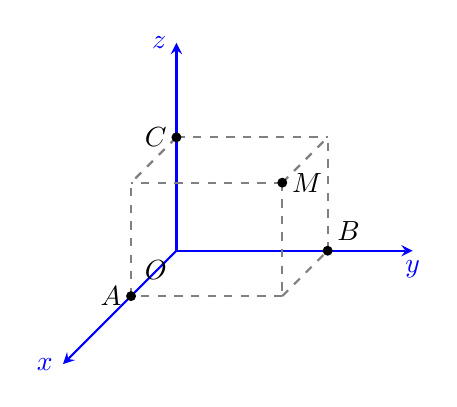
\begin{tikzpicture}[scale=1.2, >=stealth]
            % Axes
            \draw[->, thick, blue] (0,0) -- (0,2.2) node[left] {$z$};
            \draw[->, thick, blue] (0,0) -- (2.5,0) node[below] {$y$};
            \draw[->, thick, blue] (0,0) -- (-1.2,-1.2) node[left] {$x$};
            \node[below left] at (0,0) {$O$};
            
            % Coordinates of M
            \coordinate (M) at (1.12, 0.72);
            \coordinate (H) at (1.12, -0.48); % (a,b,0)
            \coordinate (C) at (0, 1.2); % (0,0,c)
            \coordinate (A) at (-0.48, -0.48); % (a,0,0)
            \coordinate (B) at (1.6, 0); % (0,b,0)
            
            % Projection faces coordinates
            \coordinate (M_yz) at (1.6, 1.2); % (0,b,c)
            \coordinate (M_xz) at (-0.48, 0.72); % (a,0,c)
            
            % Box outline projections
            \draw[dashed, thick, gray] (M) -- (H);
            \draw[dashed, thick, gray] (M) -- (M_yz);
            \draw[dashed, thick, gray] (M) -- (M_xz);
            \draw[dashed, thick, gray] (H) -- (A);
            \draw[dashed, thick, gray] (H) -- (B);
            \draw[dashed, thick, gray] (C) -- (M_yz);
            \draw[dashed, thick, gray] (C) -- (M_xz);
            \draw[dashed, thick, gray] (B) -- (M_yz);
            \draw[dashed, thick, gray] (A) -- (M_xz);
            
            % Nodes
            \fill (M) circle (1.5pt) node[right] {$M$};
            \fill (A) circle (1.5pt) node[left] {$A$};
            \fill (B) circle (1.5pt) node[above right] {$B$};
            \fill (C) circle (1.5pt) node[left] {$C$};
        \end{tikzpicture}
    \end{minipage}
\end{center}
\end{document}